

\section{Resultados}

Se explicaran ahora los resultados que hemos obtenido usando todos los recursos explicados anteriormente:

\subsection{Human Phenotipe Ontology}

\hfill

Tras realizar una búsqueda del fenotipo a investigar, \textit{Dyscalculia}, vemos que se encuentra clasificado como \href{https://hpo.jax.org/app/browse/term/HP:0002442}{HP:0002442} con un total de 13 fenotipos de otras enfermedades asociadas y un total de 24 genes asociados a esta en HPO.

Descargamos el archivo \textit{.csv} con nuestro listado de genes, para su posterior carga en String

\subsection{String}

\hfill

Gracias a las anotaciones en HPO obtenidas, procedemos a la búsqueda de más información acerca de estos, utilizando \href{https://string-db.org}{STRING}. El resultado lo podemos ver en la figura \ref{fig:string1}.

\begin{figure}[h]
	\centering
	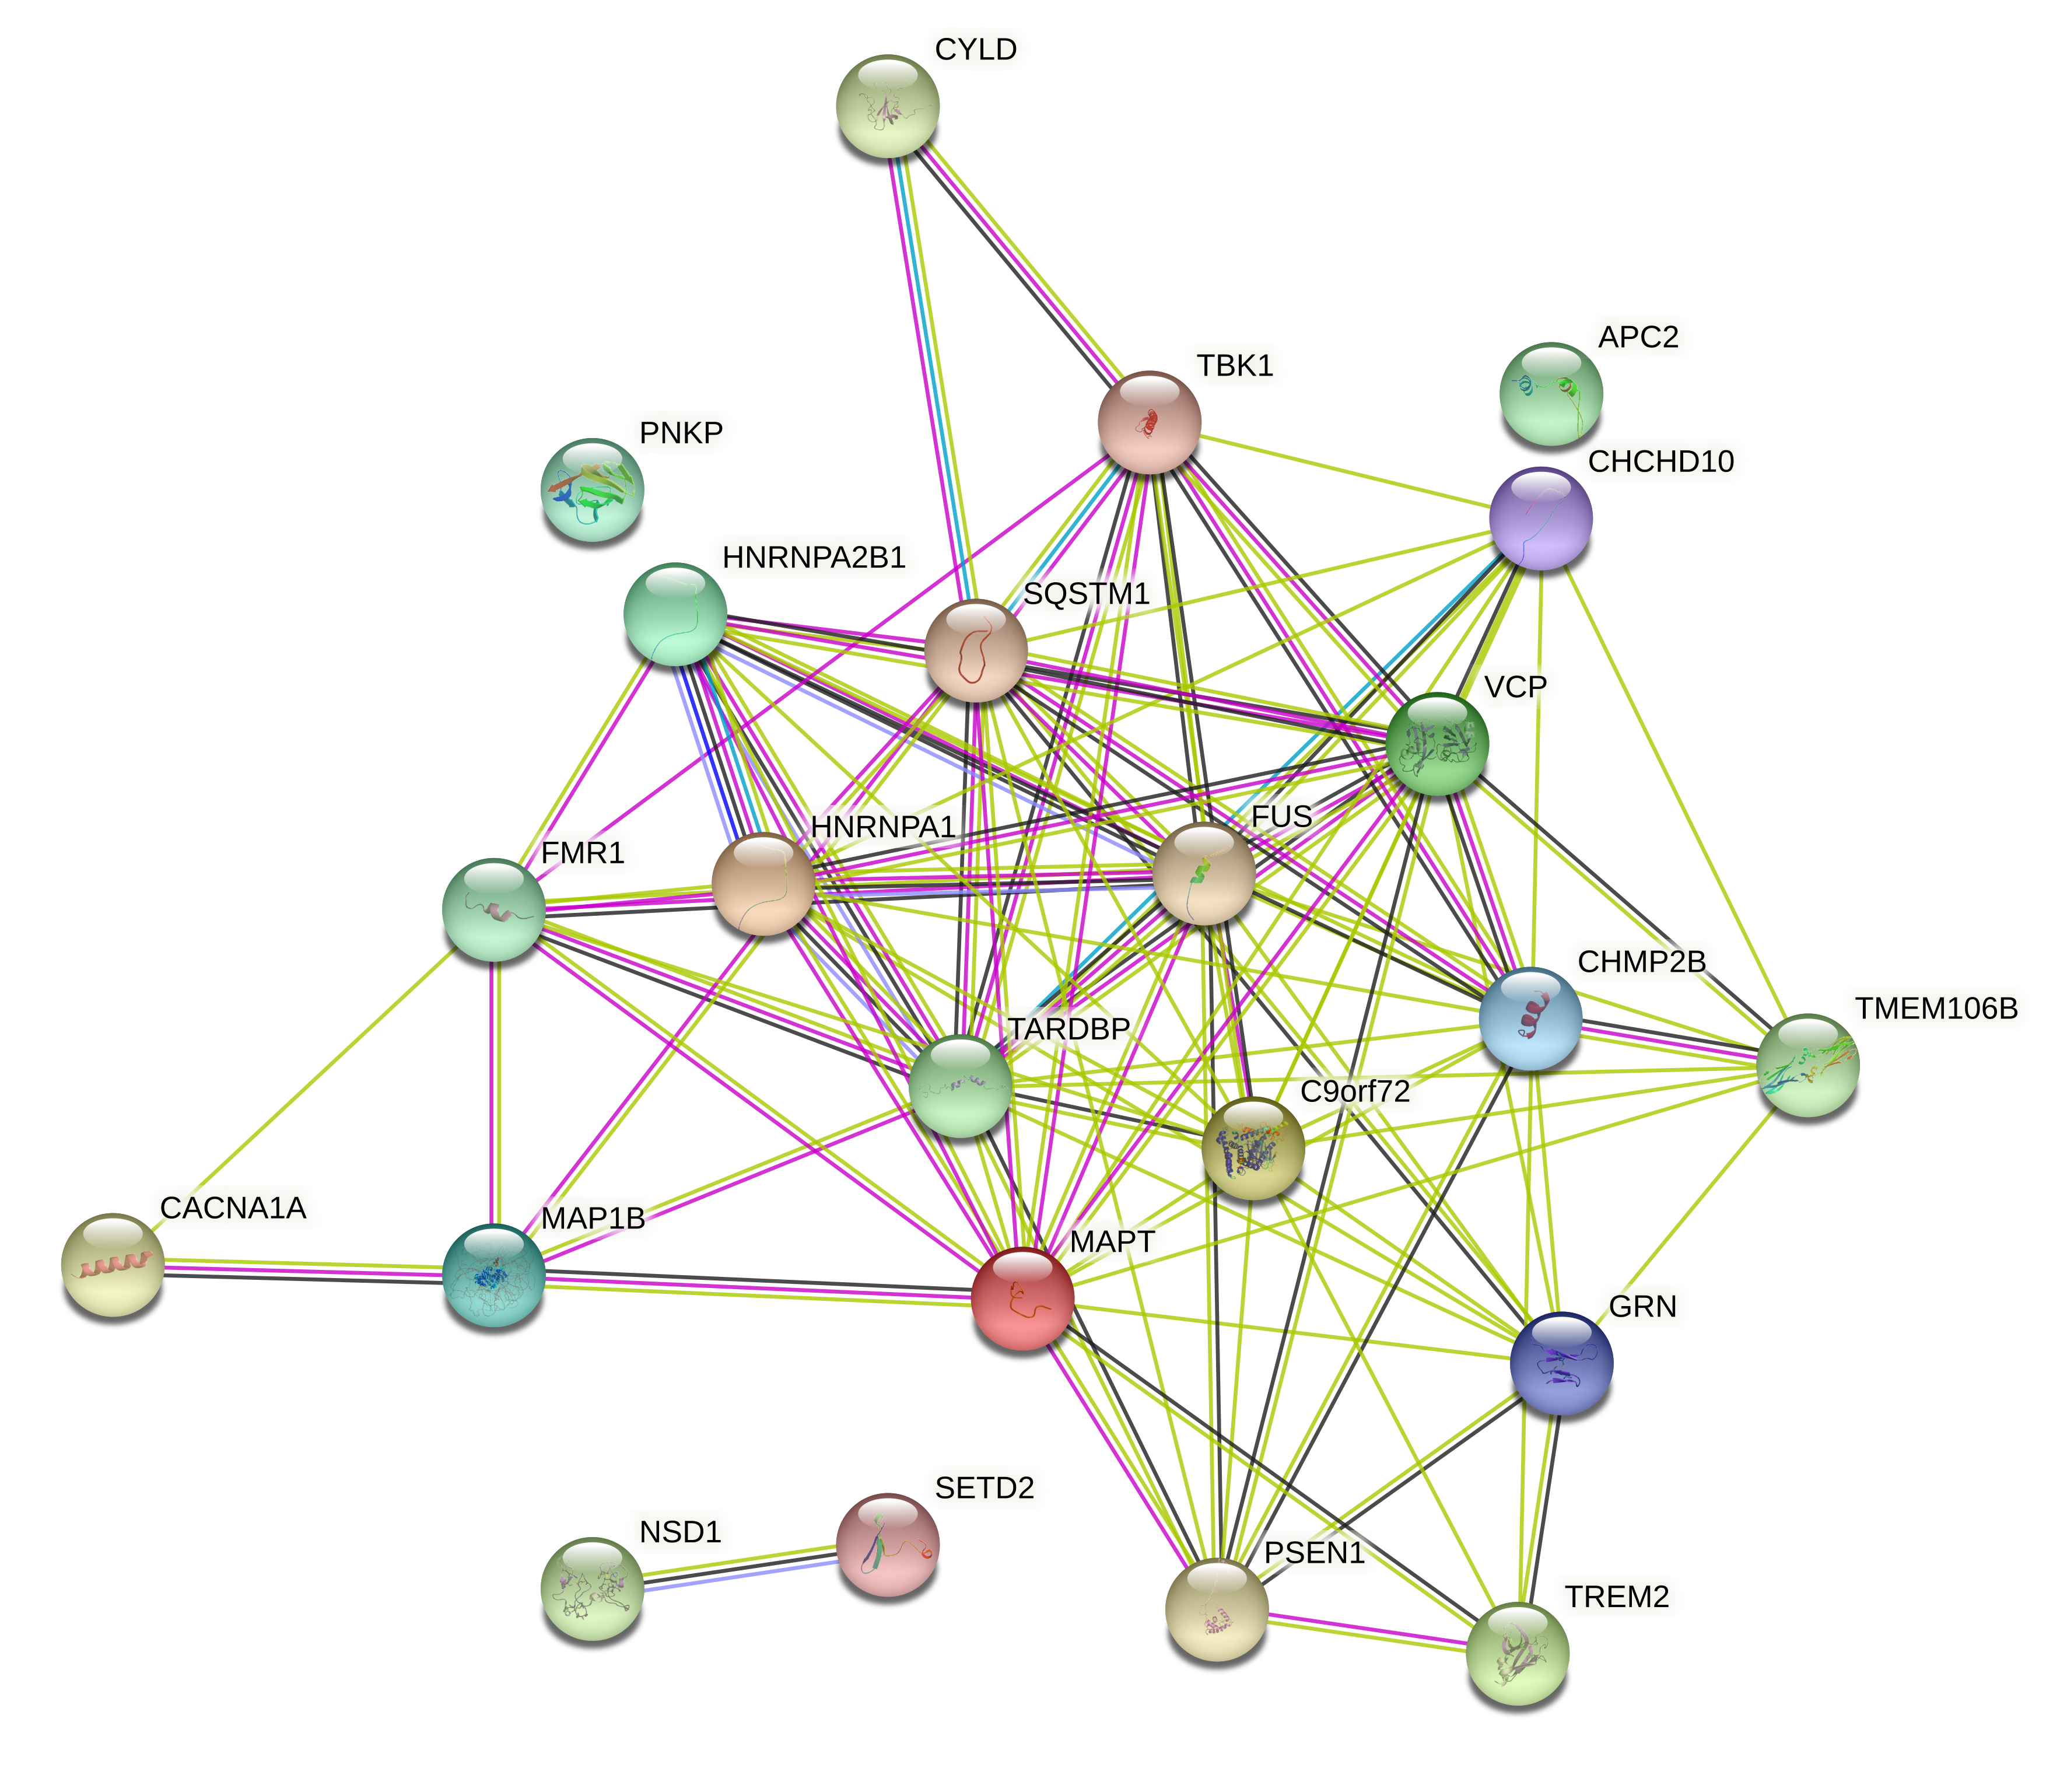
\includegraphics[width=0.90\textwidth]{figures/Gene_Relationship.png}
	\caption{Interacciones proteína-proteína a raíz de los genes relacionados. Grafo proporcionado por String.}
	\label{fig:string1}
\end{figure}

Una vez cargados los genes y sus relaciones en string, procedemos a descargar los ficheros \textit{string-node-degree.tsv} e \textit{string-interactions.tsv}.

\hfill

Se creara también un objeto network, de la librería de R \textit{stringdb}, con las siguientes características:

\hfill

Versión=11; 
Specie=9606; 
Score threshold=400

\hfill

Se usará esta red de genes humanos para buscar genes vecinos de los 24 que teníamos en un principio y realizar una propagación de red con el fin de aumentar el total de genes a estudiar que guarden directa o indirectamente una relación con nuestro fenotipo a estudiar.

\hfill

Gracias a este método el total de genes de estudio ha ascendido a 214, con esto podemos pasar al estudio de sus relaciones y funciones con una carga de trabajo mas adecuada.

Además de esto, también hemos usado String para la obtención de información adicional relacionada con la red de genes obtenida.

\subsection{igraph}

Usaremos igraph para convertir nuestro objeto network (genes originalmente relacionados con el  fenotipo mas los genes vecinos de la red general anteriormente citada) en un dataframe que sea procesable por las funciones de clustering para la división en comunidades

\hfill

\subsection{Análisis por comunidades}

Se realizan a continuación los correspondientes pasos para clusterizar nuestro conjunto en distintas comunidades y realizar el correspondiente análisis de enriquecimiento funcional a las adecuadas:

\subsubsection{LinkComm}

Tras una serie de pruebas con distintas funciones de igraph para hacer comunidades, se ha decidido usar la anteriormente citada LinkComm (con hcmethod=“single”, ya que cambiando este parametro a otros modos como “ward”, obteniamos comunidades mucho menos relevantes), que nos deja la figura \ref{fig:LinkComm1} como muestra de su trabajo sobre nuestra red de genes.

\begin{figure}[h]
	\centering
	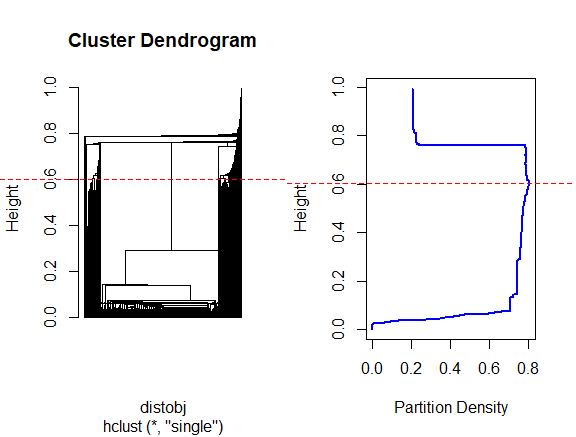
\includegraphics[width=0.60\textwidth]{figures/Grapichs_LinkComm.png}
	\caption{Dendograma del clustering realizado.Relación Altura con Densidad de particion}
	\label{fig:LinkComm1}
\end{figure}

\newpage

\hfill

Se han obtenido un total de 71 comunidades, cada una con una cantidad de los 214 nodos originales diferente. Observamos la figura \ref{fig:LinkComm2} en la que aparece un gráfico de barras con la cantidad de nodos que tienen esas comunidades.

\begin{figure}[h]
	\centering
	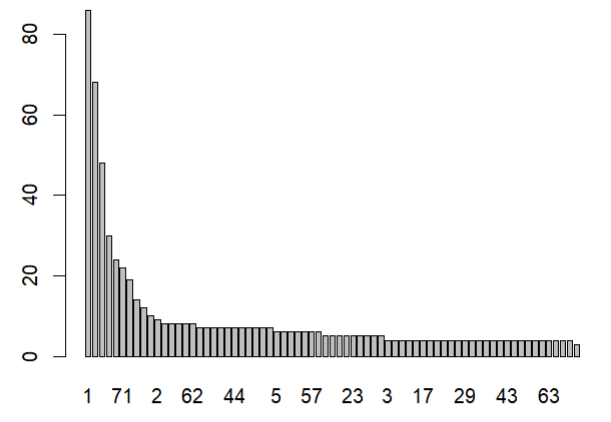
\includegraphics[width=0.70\textwidth]{figures/barplot_communities.PNG}
	\caption{Cantidad de genes de cada comunidad obtenida.Barplot del objeto de LinkComm.}
	\label{fig:LinkComm2}
\end{figure}


Además podemos observar la figura \ref{fig:LinkComm3} en la que, por colores, se nos muestra la pertenencia de cada nodo de la red a cada una de las comunidades.

\begin{figure}[h]
	\centering
	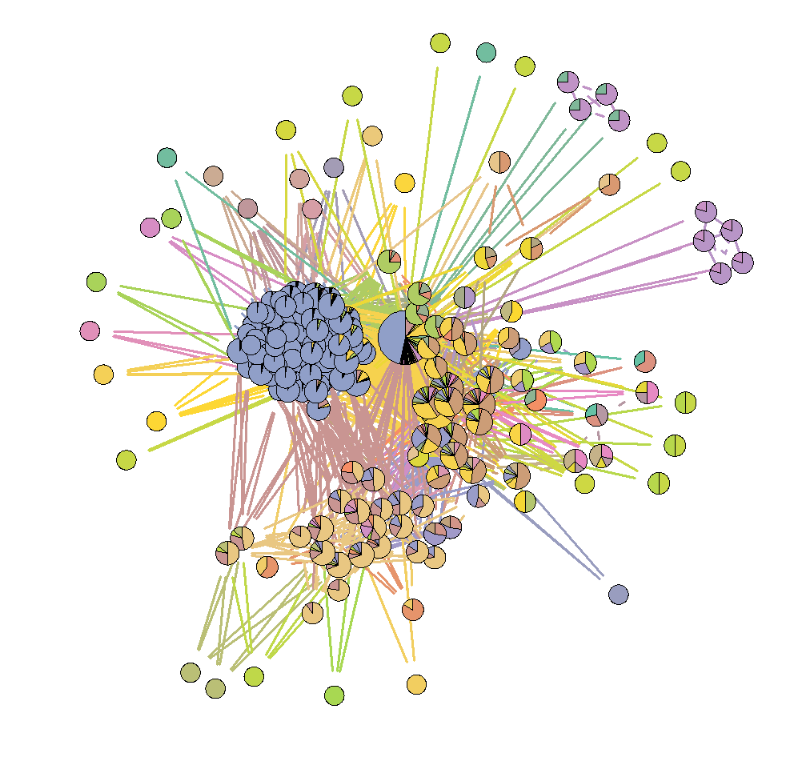
\includegraphics[width=0.65\textwidth]{figures/Grafo_Linkcomm.PNG}
	\caption{Pertenencia a las distintas comunidades de nuestra red de genes. Plot de LinkComm.}
	\label{fig:LinkComm3}
\end{figure}

\newpage

\subsection{ClusterProfiler}

\hfill

A continuación, se realizara un enriquecimiento funcional con GO (Gene Ontology) para observar las funciones implicadas en la formación de las distintas componentes celulares de las comunidades que hemos obtenido con LinkComm, con un numero de genes que suponga entre un 10/100 y un 20/100 del total de la red propagada que obtuvimos en los anteriores apartados.

\hfill

Se realizara, además, el análisis sobre la comunidad de genes originales para ver las componentes celulares relacionadas con nuestro conjunto de genes directamente vinculados a nuestro fenotipo discalculia.

\hfill


\textbf{Enriquecimiento genes originales}

 Tabla 1. Enriquecimiento del módulo de los 24 genes originales. Componentes celulares de GO en las que el conjunto de genes esta implicado.

\hfill


\begin{table}[ht]
\centering
\begin{tabular}{rlll}
  \hline
 & ID & Description & GeneRatio \\ 
  \hline
1 & GO:0036464 & cytoplasmic ribonucleoprotein granule & 6/22 \\ 
  2 & GO:0035770 & ribonucleoprotein granule & 6/22 \\ 
  3 & GO:0030426 & growth cone & 5/22 \\ 
  4 & GO:0030427 & site of polarized growth & 5/22 \\ 
  5 & GO:0010494 & cytoplasmic stress granule & 4/22 \\ 
  6 & GO:0150034 & distal axon & 5/22 \\ 
   \hline
\end{tabular}
\end{table}

\begin{table}[ht]
\centering
\begin{tabular}{rllrrlr}
  \hline
 & ID & BgRatio & pvalue & p.adjust & geneID & Count \\ 
  \hline
1 & GO:0036464 & 248/19869 & 0.00 & 0.00 & TARDBP/MAPT/VCP/FMR1/SQSTM1/C9orf72 &   6 \\ 
  2 & GO:0035770 & 265/19869 & 0.00 & 0.00 & TARDBP/MAPT/VCP/FMR1/SQSTM1/C9orf72 &   6 \\ 
  3 & GO:0030426 & 167/19869 & 0.00 & 0.00 & MAP1B/PSEN1/MAPT/FMR1/C9orf72 &   5 \\ 
  4 & GO:0030427 & 173/19869 & 0.00 & 0.00 & MAP1B/PSEN1/MAPT/FMR1/C9orf72 &   5 \\ 
  5 & GO:0010494 & 84/19869 & 0.00 & 0.00 & TARDBP/VCP/FMR1/C9orf72 &   4 \\ 
  6 & GO:0150034 & 278/19869 & 0.00 & 0.00 & MAP1B/PSEN1/MAPT/FMR1/C9orf72 &   5 \\ 
   \hline
\end{tabular}
\end{table}

\newpage

\textbf{Enriquecimiento genes de la comunidad 70}

 Tabla 2. Enriquecimiento del módulo de la comunidad obtenida con linkcomm número 70 (48 genes). Componentes celulares de GO en las que el conjunto de genes esta implicado.

\hfill

\begin{table}[ht]
\centering
\begin{tabular}{rlll}
  \hline
 & ID & Description & GeneRatio \\ 
  \hline
1 & GO:0035578 & azurophil granule lumen & 26/48 \\ 
  2 & GO:0005766 & primary lysosome & 27/48 \\ 
  3 & GO:0042582 & azurophil granule & 27/48 \\ 
  4 & GO:0005775 & vacuolar lumen & 26/48 \\ 
  5 & GO:0034774 & secretory granule lumen & 26/48 \\ 
  6 & GO:0060205 & cytoplasmic vesicle lumen & 26/48 \\ 
   \hline
\end{tabular}
\end{table}

\begin{table}[ht]
\centering
\begin{tabular}{rllrrr}
  \hline
 & ID & BgRatio & pvalue & p.adjust & Count \\ 
  \hline
1 & GO:0035578 & 91/19869 & 0.00 & 0.00 &  26 \\ 
  2 & GO:0005766 & 155/19869 & 0.00 & 0.00 &  27 \\ 
  3 & GO:0042582 & 155/19869 & 0.00 & 0.00 &  27 \\ 
  4 & GO:0005775 & 176/19869 & 0.00 & 0.00 &  26 \\ 
  5 & GO:0034774 & 322/19869 & 0.00 & 0.00 &  26 \\ 
  6 & GO:0060205 & 325/19869 & 0.00 & 0.00 &  26 \\ 
   \hline
\end{tabular}
\end{table}


\begin{table}[ht]
\centering
\begin{tabular}{rll}
  \hline
 & ID & geneID \\ 
  \hline
1 & GO:0035578 & TUBB/TUBB4B/PRDX6/ANXA2/DYNC1H1/ARG1/VCP/CAP1/PRKCD/RNASET2/IST1/ELANE \\ 
  2 & GO:0005766 & PSEN1/TUBB/TUBB4B/PRDX6/ANXA2/DYNC1H1/ARG1/VCP/CAP1/PRKCD/RNASET2/IST1/ELANE \\ 
  3 & GO:0042582 & PSEN1/TUBB/TUBB4B/PRDX6/ANXA2/DYNC1H1/ARG1/VCP/CAP1/PRKCD/RNASET2/IST1/ELANE \\ 
  4 & GO:0005775 & TUBB/TUBB4B/PRDX6/ANXA2/DYNC1H1/ARG1/VCP/CAP1/PRKCD/RNASET2/IST1/ELANE \\ 
  5 & GO:0034774 & TUBB/TUBB4B/PRDX6/ANXA2/DYNC1H1/ARG1/VCP/CAP1/PRKCD/RNASET2/IST1/ELANE \\ 
  6 & GO:0060205 & TUBB/TUBB4B/PRDX6/ANXA2/DYNC1H1/ARG1/VCP/CAP1/PRKCD/RNASET2/IST1/ELANE \\ 
   \hline
\end{tabular}
\end{table}

\newpage

\textbf{Enriquecimiento genes de la comunidad 33}

 Tabla 3. Enriquecimiento del módulo de la comunidad obtenida con linkcomm número 33 (30 genes). Componentes celulares de GO en las que el conjunto de genes esta implicado.

\hfill

\begin{table}[ht]
\centering
\begin{tabular}{rlll}
  \hline
 & ID & Description & GeneRatio \\ 
  \hline
1 & GO:0035578 & azurophil granule lumen & 25/29 \\ 
  2 & GO:0034774 & secretory granule lumen & 29/29 \\ 
  3 & GO:0060205 & cytoplasmic vesicle lumen & 29/29 \\ 
  4 & GO:0031983 & vesicle lumen & 29/29 \\ 
  5 & GO:0005775 & vacuolar lumen & 26/29 \\ 
  6 & GO:0005766 & primary lysosome & 25/29 \\ 
   \hline
\end{tabular}
\end{table}

\begin{table}[ht]
\centering
\begin{tabular}{rllrrr}
  \hline
 & ID & BgRatio & pvalue & p.adjust & Count \\ 
  \hline
1 & GO:0035578 & 91/19869 & 0.00 & 0.00 &  25 \\ 
  2 & GO:0034774 & 322/19869 & 0.00 & 0.00 &  29 \\ 
  3 & GO:0060205 & 325/19869 & 0.00 & 0.00 &  29 \\ 
  4 & GO:0031983 & 327/19869 & 0.00 & 0.00 &  29 \\ 
  5 & GO:0005775 & 176/19869 & 0.00 & 0.00 &  26 \\ 
  6 & GO:0005766 & 155/19869 & 0.00 & 0.00 &  25 \\ 
   \hline
\end{tabular}
\end{table}

\begin{table}[ht]
\centering
\begin{tabular}{rll}
  \hline
 & ID & geneID \\ 
  \hline
1 & GO:0035578 & RETN/MPO/CTSC/PRTN3/TRAPPC1/TOLLIP/ANXA2/ARG1/S100A7/DPP7 \\ 
  2 & GO:0034774 & CTSZ/RETN/MPO/CTSC/PRTN3/CTSD/CHI3L1/TRAPPC1/TOLLIP/SLPI/ANXA2/ARG1/S100A7/DPP7\\ 
  3 & GO:0060205 & CTSZ/RETN/MPO/CTSC/PRTN3/CTSD/CHI3L1/TRAPPC1/TOLLIP/SLPI/ANXA2/ARG1/S100A7/DPP7\\ 
  4 & GO:0031983 & CTSZ/RETN/MPO/CTSC/PRTN3/CTSD/CHI3L1/TRAPPC1/TOLLIP/SLPI/ANXA2/ARG1/S100A7/DPP7 \\ 
  5 & GO:0005775 & RETN/MPO/CTSC/PRTN3/CTSD/TRAPPC1/TOLLIP/ANXA2/ARG1/S100A7/DPP7 \\ 
  6 & GO:0005766 & RETN/MPO/CTSC/PRTN3/TRAPPC1/TOLLIP/ANXA2/ARG1/S100A7/DPP7\\ 
   \hline
\end{tabular}
\end{table}

\newpage

\textbf{Enriquecimiento genes de la comunidad 48}

 Tabla 4. Enriquecimiento del módulo de la comunidad obtenida con linkcomm número 48 (24 genes). Componentes celulares de GO en las que el conjunto de genes esta implicado.

\hfill

\begin{table}[ht]
\centering
\begin{tabular}{rlll}
  \hline
 & ID & Description & GeneRatio \\ 
  \hline
1 & GO:0043025 & neuronal cell body & 10/22 \\ 
  2 & GO:0150034 & distal axon & 8/22 \\ 
  3 & GO:0030426 & growth cone & 7/22 \\ 
  4 & GO:0030427 & site of polarized growth & 7/22 \\ 
  5 & GO:0045121 & membrane raft & 8/22 \\ 
  6 & GO:0098857 & membrane microdomain & 8/22 \\ 
   \hline
\end{tabular}
\end{table}

\begin{table}[ht]
\centering
\begin{tabular}{rllrrr}
  \hline
 & ID & BgRatio & pvalue & p.adjust & Count \\ 
  \hline
1 & GO:0043025 & 497/19869 & 0.00 & 0.00 &  10 \\ 
  2 & GO:0150034 & 278/19869 & 0.00 & 0.00 &   8 \\ 
  3 & GO:0030426 & 167/19869 & 0.00 & 0.00 &   7 \\ 
  4 & GO:0030427 & 173/19869 & 0.00 & 0.00 &   7 \\ 
  5 & GO:0045121 & 326/19869 & 0.00 & 0.00 &   8 \\ 
  6 & GO:0098857 & 327/19869 & 0.00 & 0.00 &   8 \\ 
   \hline
\end{tabular}
\end{table}

\begin{table}[ht]
\centering
\begin{tabular}{rll}
  \hline
 & ID & geneID \\ 
  \hline
1 & GO:0043025 & APOE/SOD1/APP/LRRK2/PSEN1/SNCA/MAPT/PSEN2/TNF/C9orf72 \\ 
  2 & GO:0150034 & APP/LRRK2/PSEN1/SNCA/MAPT/PSEN2/PRNP/C9orf72 \\ 
  3 & GO:0030426 & APP/LRRK2/PSEN1/SNCA/MAPT/PSEN2/C9orf72 \\ 
  4 & GO:0030427 & APP/LRRK2/PSEN1/SNCA/MAPT/PSEN2/C9orf72 \\ 
  5 & GO:0045121 & APP/LRRK2/PSEN1/MAPT/PSEN2/TREM2/PRNP/TNF \\ 
  6 & GO:0098857 & APP/LRRK2/PSEN1/MAPT/PSEN2/TREM2/PRNP/TNF \\ 
   \hline
\end{tabular}
\end{table}

\textbf{}